% Rangefinding Hardware

\chapter{Rangefinding Hardware} % Main chapter title

\label{RangefindingHardware}

\section{Wireless Communications}
At the start of the project, it was determined that a technology would need to be chosen to handle wireless communications for ranging purposes. A number of options were considered. The ideal technology would:
\begin{itemize}
	\item Be inexpensive.
	\item Have good range for in-door use.
	\item Allow for extremely precise measurements of time. Due to the speed of light, a nanosecond of error in timing calculations would lead to approximately 30cm of error in the calculated distance.
	\item Be small. As tags are attached to cellphones, they must be small.
\end{itemize}

\subsection{Bluetooth in Phones: A Failed Approach}
(TODO REMOVE THIS OR APPENDIX IT WE SHOULD FOCUS ON OUR END PRODUCT AS PER AIDEN) 

Originally, the goal was to use Bluetooth for ranging. The reason for this was that Android cellphones, which usually have Bluetooth transceivers, could be used for tags and anchors. This would save a large amount of time, as cellphones include batteries, are easy to program, and almost everyone has one (which would make letting people use our project as easy as downloading an app). We would just need to put a few phones running our app around a room, and we'd get ranging. Others were able to use Bluetooth to form indoor positioning systems \cite{BluetoothIndoor}.

Unfortunately, it became clear early on that Bluetooth -- specifically, Bluetooth used on Android cellphones -- was not suitable. 

There were two ways to use Bluetooth for ranging, and we checked the viability of both: 

\begin{itemize}
	\item RSSI (received signal strength indicator), which is essentially a measure of how strong a received signal is. Because signal power drops off with the square of distance, RSSI can be used to determine distance from a cellphone. Indeed, there this is a cellphone app to do just that on the Google Play Store. Measurements showed that this was method had very low range, was very noisy (power levels varied wildly), and had a large latency between measurements. As well, RSSI values are not standard among cellphones, requiring many calibrations for each model of phone used. Due to these factors, it was determined that using RSSI for distance measurements was not well suited for the fine-grained location tracking this project sought. 
	\item Time-of-flight measurements. Experiments showed that the time it took to send a Bluetooth message itself through the Android OS suffered massive variance of milliseconds (ADD IN APPENDIX CITATION WITH OUR CODE?), which would lead to 300 km of error in calculated distances! Android does not have any guarantees on timing, and does not allow low-level programming access to its internals. This method was proven unworkable.
\end{itemize}

With all the avenues to use Bluetooth exhausted, the idea of using phones and their Bluetooth transceivers was rejected.

\subsection{Ultra-wideband and the DWM1000}
After doing some research, we discovered the Decawave DWM1000 ultra-wideband transceiver. This chip is advertised as specifically being suited for ranging applications. It uses ultra-wideband technology rather than Bluetooth, Wi-Fi, or similar technologies.

Ultra-wideband, in contrast to Wi-Fi and other radio technologies, occupies a large bandwidth and transmits information via high-bandwidth pulses. Ultra-wideband is suited to tracking applications due to its resistance to multipath propagation, a phenomenon where signals reflect off of surfaces and thus reach the antennae via multiple paths (causing interference). An in-depth look at ultra-wideband is beyond the scope of this report, but interested readers might look more at (INCLUDE SOURCES HERE!!!).

The DWM1000 is advertised as:
\begin{itemize}
	\item Allowing one to locate objects with up to 10cm accuracy.
	\item Having a range of up to 290m.
	\item Having a data rate of up to 6.8Mb/s.
	\item Having a small physical size. 
\end{itemize}

As well, there was an already an open source library written to use it with an Arduino, which would allow us to quickly prototype with the chip and ensure it would fit for our application.

Because these qualities satisfied our requirements, the DWM1000 was chosen for the foundational technology of the ranging part of the project. 

\section{Design of the Hardware}
The hardware design for tags is an Arduino Pro Mini 3.3V connected to a DWM1000 over a PCB. 

\subsection{The Microcontroller}
To interface with the DWM1000, a microcontroller was needed. The Arduino Pro Mini 3.3V was chosen because:
\begin{itemize}
	\item Others had used it with the DWM1000 and had good results \cite{LPSMini}.
	\item Group members had previous experience with programming Arduinos.
	\item It was inexpensive (\$13 before tax).
	\item It worked off of 3.3V power, which was what the DWM1000 required. This obviated the need for voltage stepping.
	\item It was capable of floating point math, which is useful for asynchronous two-way ranging. As well, barely any processing power or RAM was perceived to be needed (this was not quite true). Each microcontroller only needed to hold a small number of timestamps, so the small amount of memory and slow processor was not important.
	\item It had a small physical size. As tags are attached to cellphones, they must be small.
	\item Batteries would not be needed to power tags, since power could be delivered via USB from the cellphone. This further simplified the design and kept costs low, though the USB cables required to connect the Arduinos ended up wiping out a lot of the cost savings.
\end{itemize}

The downside of the Pro Mini was that it required a lot of soldering. 

\subsection{Anchors}
\begin{figure}
	\centering
	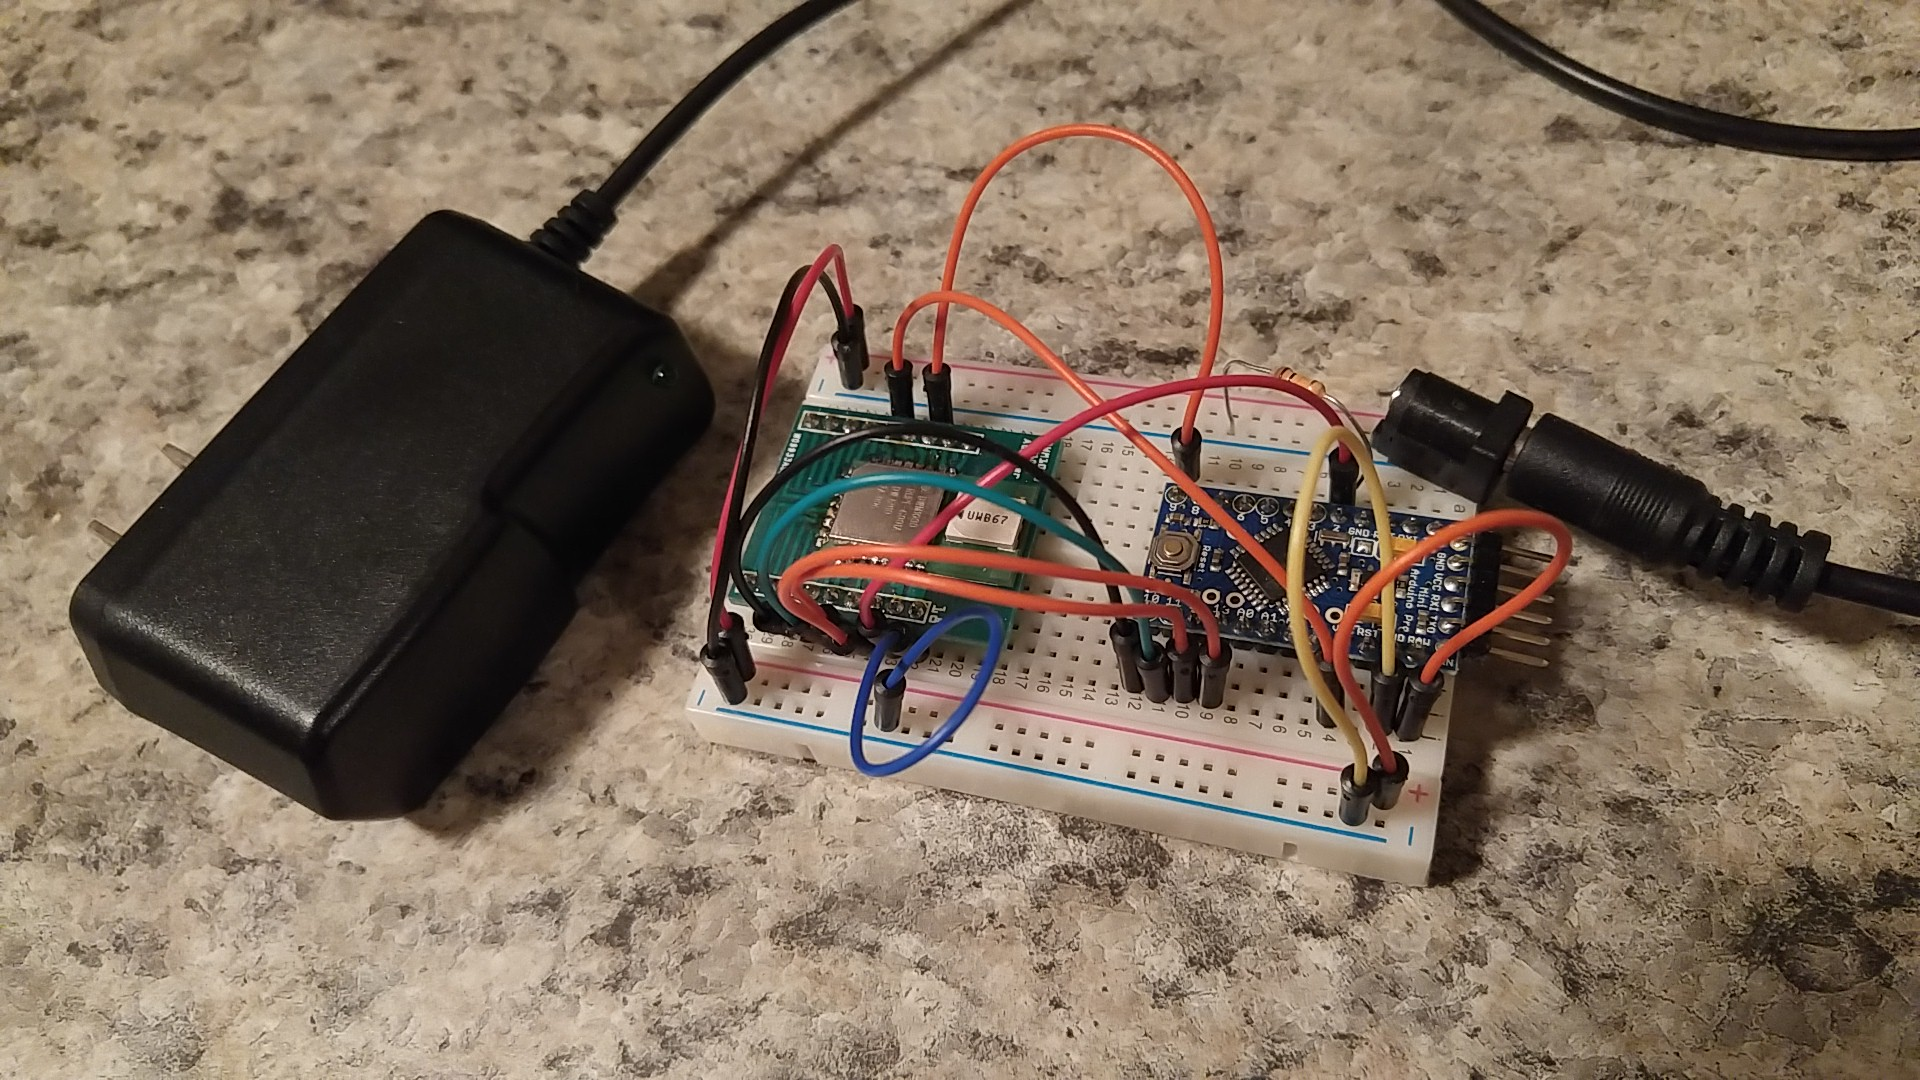
\includegraphics[width=\linewidth]{Figures/Anchor.jpg}
	\decoRule
	\caption{An anchor built on a breadboard using Thomas Trojer's PCB design \cite{ThotroGithub}. The DWM1000 is on the left, and the Arduino is on the right.}
	\label{fig:Anchor}
\end{figure}

The anchors made for use with this project were made on a breadboard and based on the design by Thomas Trojer in his \code{arduino-dw1000} library \cite{ThotroGithub}. A PCB design was included with this library which allowed a DWM1000 to be used with a breadboard. This PCB design was used in order to quickly prototype and determine whether the DWM1000 and Arduino would be feasible and meet the requirements for the project. Four anchors were constructed using these PCBs. An anchor can be seen in Figure~\ref{fig:Anchor}.

As anchors are assumed to be stationary, and the project is intended to be used indoors, it was determined that the anchors could be powered via a standard electrical outlet. Designs using batteries were considered, but as the added flexibility in placement of the anchors was of marginal benefit, and there was added complexity and maintenance required to deal with the batteries, the option was not pursued.

To save costs and time, the anchors' designed stayed constant throughout the project. There was only marginal benefit to designing a PCB, as their size was mostly irrelevant and their performance would not be improved.

\subsection{Tags}
\begin{figure}
	\centering
	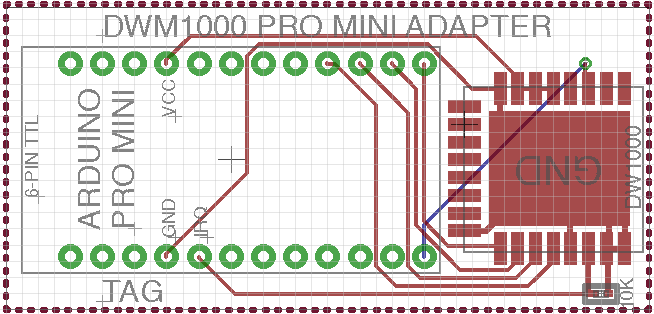
\includegraphics[width=\linewidth]{Figures/PCB.png}
	\decoRule
	\caption{The design for the tag PCB in EAGLE.}
	\label{fig:PCB}
\end{figure}

\begin{figure}
	\centering
	\includegraphics[width=\linewidth]{Figures/Tag.jpg}
	\decoRule
	\caption{A soldered tag.}
	\label{fig:Tag}
\end{figure}
The tags made for use with this project were required to be small enough to comfortably attach on a headset or cellphone. As a breadboard was too large, a custom PCB was designed.

Several designs were considered for the PCB connecting the Arduino and DWM1000. The most important factors were size and cost.

Several designs were considered at first:
\begin{itemize}
	\item The first idea considered was to place the Arduino and DWM on top of each other, resulting in the smallest possible size. However, the physical dimensions of the two components made this impossible. 
	\item Another possibility was to place each component on opposite sides of the PCB, but the Arduino's design demanded breakout headers to solder it into the board, which meant the PCB had to have holes drilled, which again meant that the physical dimensions of the two components interfered.
	\item Yet another idea was to make two PCBs. The Arduino would connect to a PCB above it, and that PCB would connect to a board above it with the DWM1000 soldered to it. Because it was layered, the pins connecting the layers could be arranged such that the Arduino and DWM1000 were essentially above each other, but without the locations of their pins interfering with each other. This design was abandoned because the breakout pins would add a large amount of vertical length, it was twice as expensive, and because it was much more complex to design.
	\item The final idea considered was to have the Arduino and DWM1000 just be placed next to each other on the same side of a PCB. This design was physically realizable, the least expensive, and though it was not as compact as would be ideal, it was still relatively small.
\end{itemize}

The last idea was chosen due to the its cheap cost, simplicity of design, and satisfactory size. 

As others who had used the DWM1000 recommended it \cite{LPSMini}, the PCB was designed so the antenna would not be on the PCB.

The PCB design was done in EAGLE and ordered from PCBWay. The PCB design can be seen in Figure~\ref{fig:PCB} and a soldered tag can be seen in Figure~\ref{fig:Tag}.

\section{Arduino Software}
The software to control the DWM1000 was written in C++ in Arduino IDE. The basic code to control the DWM1000 (handling memory address constants, communication with it via SPI, and a few high-level functions like send/receive) was freely available in Thomas ``thotro'' Trojer's \texttt{arduino-dw1000} library. The library served as the foundation of our code to network the devices.

\subsection{Calculating a Delay}
\label{CalculatingADelay}
As part of the time of flight calculation, a timestamp is needed for when the message was received and for when the reply was sent. The DWM1000 does not offer a way to automatically set the time upon transmission, but does offer the ability to set a time when a message will be transmitted in the future. This timestamp can then be embedded in the message itself.

Ideally, this delay is short. However, if the delay is too short, the Arduino will not be able to transmit the data the DWM1000 should send before the timestamp is passed. This causes a silent error, and the DWM will not transmit anything. As well, the delay specified is not the delay at which the DWM1000 will begin transmitting, it is the delay that the DWM1000 will begin transmitting the data itself. There is a ``premable'' sent before any transmission to allow the other devices in the network time to wake up and begin sniffing the air and know a message is coming. This time to send the preamble lasts quite a long time (approximately 1 microsecond per symbol in the problem (ADD CITATION HERE), which adds up to almost 2 ms). This was the most difficult to solve bug that was encountered in the design of the system.

In the code, the delay before we can transmit is the sum of the:
\begin{itemize}
	\item Number of symbols in the preamble $\times$ 1\si{\micro\second} (128 is the value used here, though the DWM offers a choice of preamble length)
	\item Time required to calculate and send the timestamp using SPI, about 1000\si{\micro\second} (empirically determined)
	\item Bytes of data to transmit $\times$ 4.5\si{\micro\second}, or 85 $\times$ number of devices in the network besides this one (empirically determined)
\end{itemize}

Adding in a fudge factor of about 200\si{\micro\second}, the delay we use in code for 6 devices is roughly 1800 \si{\micro\second}.

It is important to minimize this delay so to increase the maximum frequency the system can update ranges at. The tradeoff of having a short preamble versus a long one is that a long preamble means there is less chance of a transmission being missed, at the cost of using more power and taking longer to send. The value of 128 was chosen as it was the smallest possible. Tests indicated that transmissions were not being lost enough to matter with such a short preamble.

\section{Calibrating}
DWM1000s need to be calibrated to give correct distances due to the differences in hardware. There are a number of factors affecting the DWM1000, such as temperature. Some of these factors are controlled for in software in the arduino-dw1000 library. For a detailed overview of the possible errors and how to correct for them, the reader is advised to read the relevant sections in the DW1000 User Manual \cite{DW1000UserManual}.

The primary factor which could not be controlled for by Decawave is the antenna delay. The capacitance of the hardware the DWM1000 is hooked up to can cause nanosecond-level delays in transmission (in experiments, it was found that this could cause up to several meters of error incorrectly configured). This is a constant, and is determined empirically. The antenna delay for the tags is the same and was found to be INSERT NUMBER HERE THAT WE FOUND, and the antenna delay for the anchors is roughly the same and was found to be INSERT NUMBER HERE.

These constants required a slight tweak to the DWM1000 library. INSERT LINK TO SOURCE CODE OF OUR CHANGED VERSION HERE.

\section{Operating Frequency Analysis}
\label{OperatingFrequencyAnalysis}
In order to estimate the operating frequency of the rangefinding subsystem -- that is, how many times we can get the range from all devices to a single device per second\footnote{It should be noted that this definition of operating frequency is somewhat misleading and calculates a minimum operating frequency. Because each pair of devices compute their range twice, once on each device at different points in the round, the true operating frequency of the system will be higher on average. The analysis here does not take this into account. 

In the best case scenario, this will almost double the system frequency. In the worst case scenario, where two devices are next to each other in the transmission order in a large network, the system operating frequency will barely increase. The figures given for operating frequencies will thus give a range from the minimum by the definition here to twice it.} -- we see that the frequency will be the inverse of the time taken to complete one round (the system performs one range update per device per round), assuming no lost transmissions. That is,

\[
 	f_{op} = \frac{1}{T_{round}}
\]

The time it takes a round is equal to the time it takes the devices to each parse a received message and transmit a message. Determining the time it takes to transmit a message is a little tricky to calculate due to the requirement to include the delay before the message is sent. A rough estimate of the time it takes to do a round of transmissions is:

\[
	T_{round} =  N(T_{device} + T_{prop}) + T_{end}
\]
where $N$ is the number of nodes in the network (the 4 anchors and 3 tags that were made make 7), $T_{device}$ is the time it takes a device to fully receive and transmit, $T_{prop}$ is the time it takes the message propogate (this will not be constant, but it is so small as to be ignorable in this analysis), and $T_{end}$ is the duration of the pause at the end of the round. 

We can estimate $T_{device}$ as

\[
	T_{device} \approx T_{rx} + T_{tx} + T_{txDelay}
\]
where $T_{rx}$ is the time it takes to parse a received message (7-8 ms empirically), $T_{tx}$ is the time it takes to create the packet to send to the DWM1000 (1-2 ms empirically), $T_{txDelay}$ is the delay before the ranging packet can be sent (calculated in Section~\ref{CalculatingADelay}, about 1800 \si{\micro\second}).

Putting it all together, the equation estimating the operating frequency of the system is:
\[
	T_{round} \approx N(T_{rx} + T_{tx} + T_{txDelay}) + T_{end}
\]

$T_{end}$ is implemented in the code as a dummy device which the network will never receive a message for, allowing it to expire. Perhaps unintuitively, it is not actually equal to the time it takes a normal device to be rejected. This is because, when the round ends, it will not have transmitted anything, meaning that the time it takes to parse a received message will be 0 from it and the next round will start as soon as the first device in the transmission order array can transmit. $T_{end}$, then, is about equal to $T_{tx} + T_{txDelay}$.

Plugging the above numbers into the equation, we find we should expect that a network composed of 2 devices can operate at a frequency of about 40Hz and a network of 7 devices can operate at about 13Hz. These estimates are quite close to the empirical measurements made (see Section~\ref{RangefindingResults}).

As can be seen from the equations, the system is primarily bottlenecked by the speed at which messages can be processed and transmitted. These numbers are well above what the minimum requirements for the system, but they are below an ideal 60Hz (at which point the updates would be so smooth as to seem mostly continuous to the human eye and there would be marginal benefit to improving the frequency). Originally, it was thought that the Arduino's speed would not matter, but this turned out to not be the case. Future work on this project would benefit from finding a faster microcontroller, or perhaps offloading all processing to the cell phone each tag is hooked up to. 

An optimization that was considered and rejected due to time constraints was offloading only the time-of-flight calculation to the cell phones, instead transmitting timestamps instead of calculated ranges in the ranging packets. The Arduino Pro Mini was found to take roughly 1ms to calculate each range. Implementing this would increase the operating frequency by about 1Hz - not enough to justify any time spent on it.

\section{Results}
\label{RangefindingResults}
Results showed that the DWM1000 was close to as accurate as Decawave claimed (within 10cm). Of note, sometimes the reported ranges would glitch and be off by a meter or more. Table~\ref{tab:RangefindingAccuracy} shows the accuracy of the system. Though the accuracy of the rangefinding system was not a direct requirement of the project as a whole, the accuracy of the rangefinding system translates into accuracy of the position calculating system and thus the accuracy of the markers on the AR display.

\begin{table}
\caption{Accuracy of the rangefinding subsystem. Experiment performed with two tags lying on the ground and a tape measure.}
\label{tab:RangefindingAccuracy}
\centering
\begin{tabular}{l l l}
\toprule
\tabhead{Actual Distance} & \tabhead{Reported Distance} & \tabhead{Standard Deviation} \\
\midrule
TBD & TBD & TBD \\
\bottomrule \\
\end{tabular}
\end{table}

The operating frequency was close to the values predicted by the theory in Section~\ref{OperatingFrequencyAnalysis}. Predicted and actual values can be found in Table~\ref{tab:RangefindingFrequency}.

The max range between nodes was not determined due to space limitations but was at least 10m. The DWM1000 should get at least 60m if there are no obstructions \cite{DWM1000UserManual}.

\begin{table}
\caption{The frequencies of the rangefinding subsystem for various numbers of devices in the network. Experimented performed by placing an increasing number of devices in a network and calculating the duration between range reports from node 1 to node 2.}
\label{tab:RangefindingFrequency}
\centering
\begin{tabular}{c c c}
\toprule
\tabhead{Number of Devices} & \tabhead{Round Time (\si{\micro \second})} & \tabhead{Frequency (Hz)} \\
\midrule
2 & 37000 & 27 \\
3 & 58000 & 17.2 \\
4 & 86000 & 11.6 \\
5 & 93000 & 10.8 \\
6 & 156000 & 6.4 \\
7 & 170000 & 5.9 \\
\bottomrule
\end{tabular}
\end{table}
